\documentclass[a4paper]{article}
\usepackage{xcolor}
\usepackage{amsmath}
\usepackage{mathtools}
\usepackage{siunitx}
\usepackage{booktabs}

\title{Comparison of Terrain Following and Cut Cell Grids with a Non-Hydrostatic Model}
\author{James Shaw}
\date{TODO}

\begin{document}
\newcommand{\TODO}[1]{\textcolor{purple}{TODO: \emph{#1}}}
\newcommand{\textcite}[1]{\textbf{#1}}

\maketitle

\section{Results}

\begin{itemize}
	\item Horizontal advection
	\item \TODO{Maybe wobblyTracerAdvection}
	\item Resting atmosphere
	\item Gravity waves
\end{itemize}

\begin{figure}
	btf-cubicUpwindCPCFit-divFree \\
	\input{../advectTracer-horizontal-btf-cubicUpwindCPCFit-divFree/tracer-contour}
	\input{../advectTracer-horizontal-btf-cubicUpwindCPCFit-divFree/error-contour}

	schaer-4thorder \\
	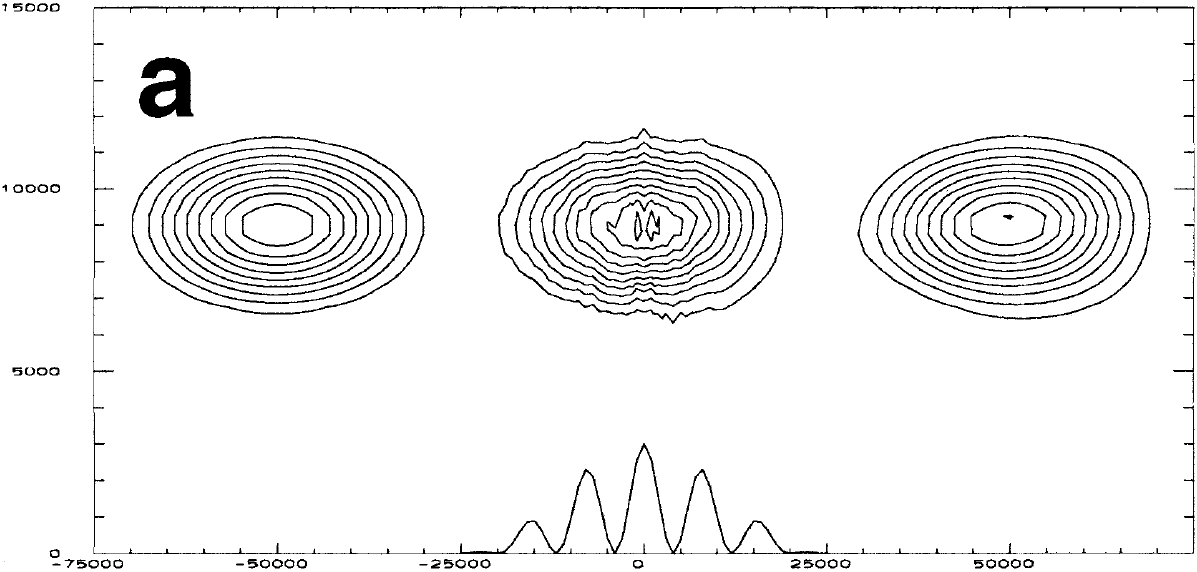
\includegraphics[height=1.5in]{schaer-btf-4thorder.png}
	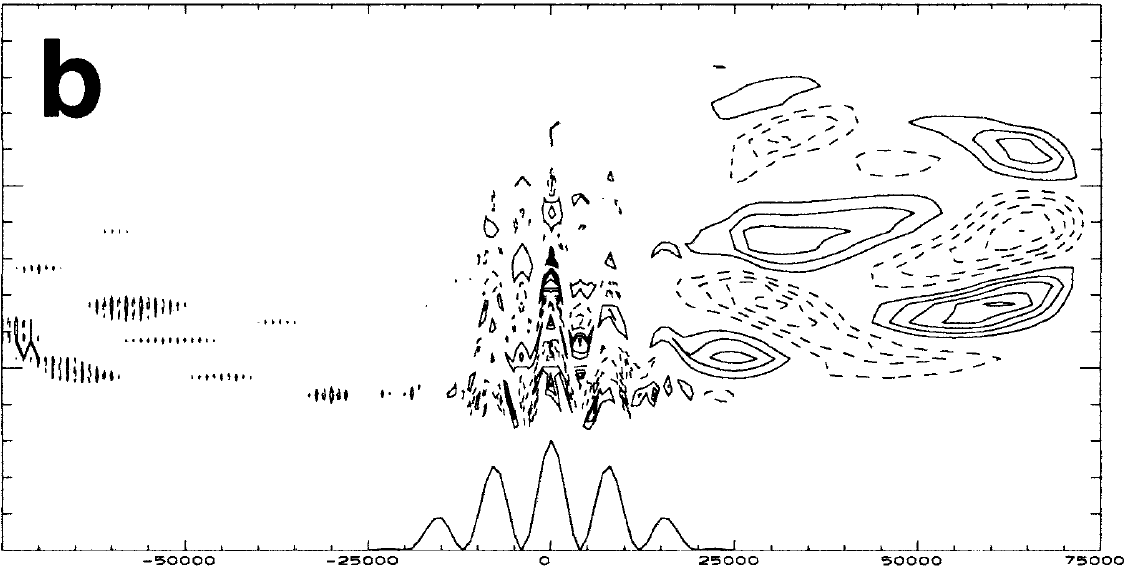
\includegraphics[height=1.5in]{schaer-btf-4thorder-error.png}
%
	\caption{Comparing our BTF cubicUpwindCPCFit result with Schaer's 4th order result}
	\label{fig:advection}
\end{figure}

\begin{table}
\centering
\begin{tabular}{ l l l l l l }
\toprule
& \multicolumn{3}{c}{Cubic upwind-biased} & \multicolumn{2}{c}{Sch\"ar 4th order} \\
& $\ell^2$ error & min & max & min & max \\
\midrule
Analytic  & 0 & 0 & 1 & \multicolumn{1}{c}{---} & \multicolumn{1}{c}{---} \\
BTF 	  & TODO & TODO & TODO & \num{-0.058} & \num{1.001} \\
SnapCol   & TODO & TODO & TODO & \multicolumn{1}{c}{---} & \multicolumn{1}{c}{---} \\
noOrography & TODO & TODO & TODO & \num{-0.002} & \num{0.984} \\
\bottomrule
\end{tabular}
%
\caption{Min, max and error norms compared with \textcite{schaer2002}}
\label{tab:advection-stats}
\end{table}

\begin{figure}
	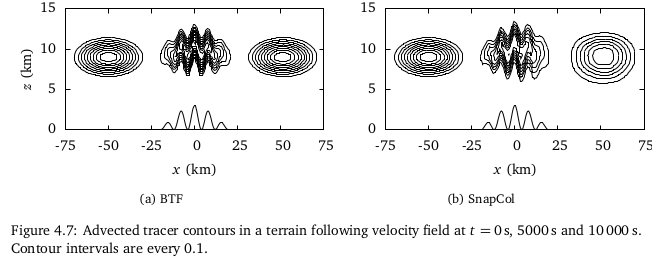
\includegraphics[height=2in]{wobblyTracerAdvection.png}
%
	\caption{tracer advection in terrain following velocity field}
	\label{fig:wobblyTracerAdvection}
\end{figure}

\begin{figure}
	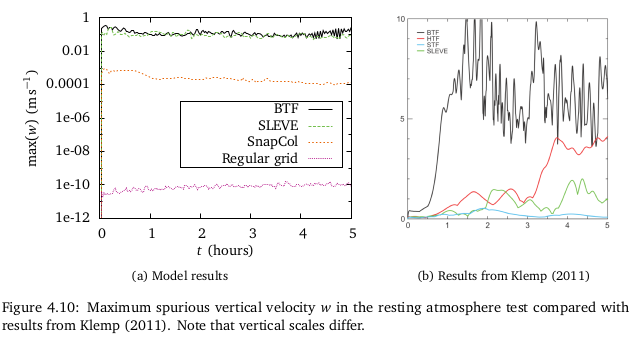
\includegraphics[height=3in]{resting-atmosphere-w.png}
%
	\caption{Comparing our results with \textcite{klemp2011}'s}
	\label{fig:resting}
\end{figure}

\begin{figure}
	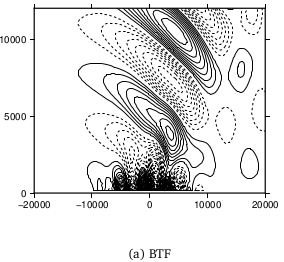
\includegraphics[height=2in]{gw-w-btf.png}
	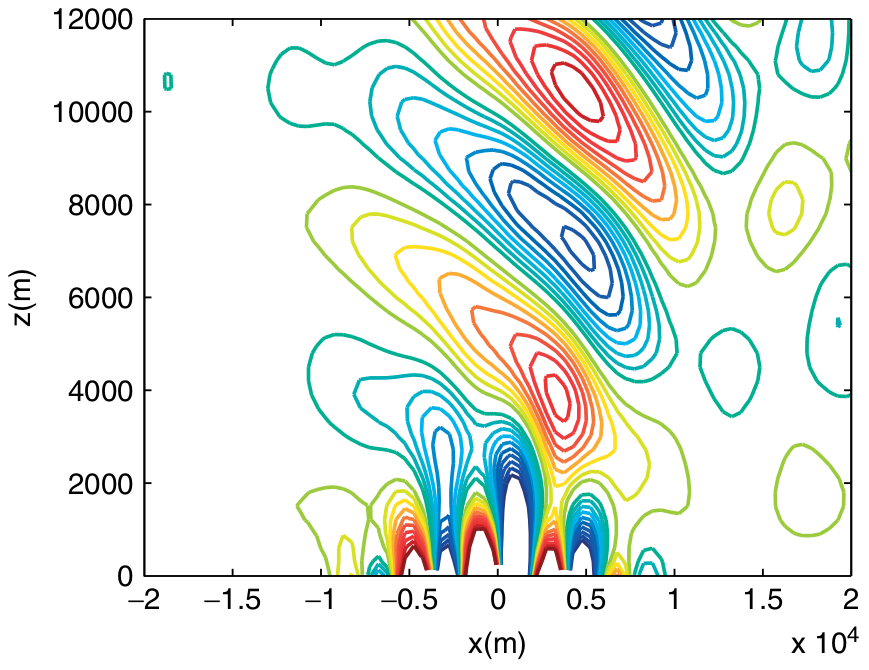
\includegraphics[height=2in]{melvin-7a.png}
%
	\caption{Gravity wave vertical velocities and thermal anomalies from initial thermal profile}
	\label{fig:gw-w}
\end{figure}

\begin{figure}
	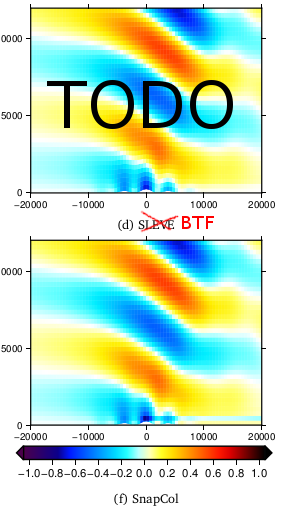
\includegraphics[height=3in]{gw-theta.png}
	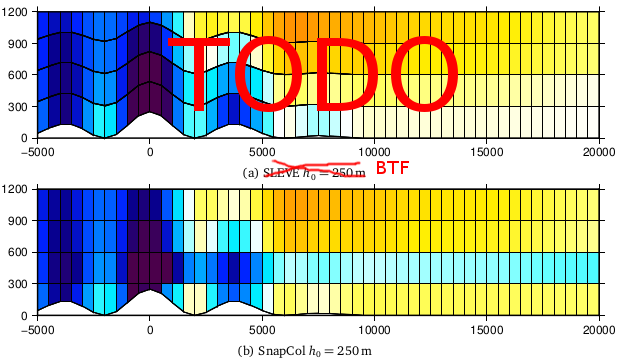
\includegraphics[height=3in]{gw-theta-zoom.png}
%
	\caption{Gravity wave thermal anomalies from initial thermal profile}
	\label{fig:gw-theta}
\end{figure}

\begin{figure}
	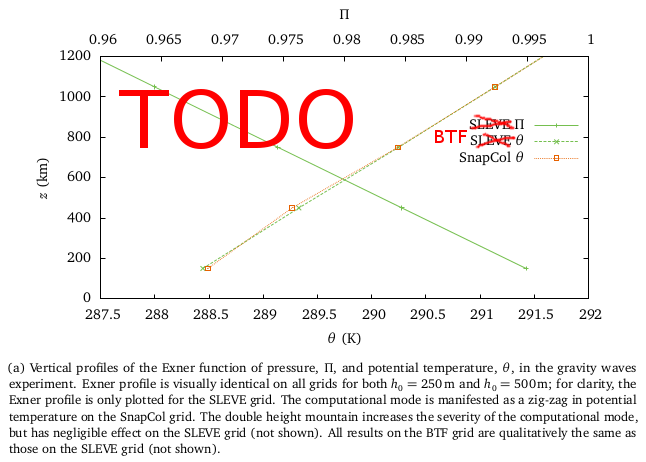
\includegraphics[height=3in]{gw-exner-theta.png}
%
	\caption{Vertical sample line of Exner function of pressure and theta to demonstrate Lorenz computational mode}
	\label{fig:gw-exner-theta}
\end{figure}

\section{Conclusions}
\begin{enumerate}
	\item BTF grid isn't as bad as people say it is.  We found that:
	\begin{itemize}
		\item Upwind-biased cubic advection scheme accurately advects a tracer in non-divergent flows (Figure~\ref{fig:advection}, Table~\ref{tab:advection-stats})
		\item Advection in a TF velocity field, if we include it, gives better results on BTF than SnapCol (Figure~\ref{fig:wobblyTracerAdvection})
		\item spurious vertical velocities are small in resting atmosphere (Figure~\ref{fig:resting})  Could also compare with \textcite{zaengl2012}, \textcite{good2014}
		\item gravity waves results visually as good as reference solution from \textcite{melvin2010} (figure~\ref{fig:gw-w})
	\end{itemize}

	\item Cut cell grids can be worse than TF grids:
	\begin{itemize}
		\item Lorenz computational mode found on SnapCol grid only (figure~\ref{fig:gw-theta}, \ref{fig:gw-exner-theta})
	\end{itemize}
\end{enumerate}

Miscellany:
\begin{itemize}
	\item Advection accuracy depends on alignment of the flow with grid layers
	\item Little/no evidence of small cell problem in GW test
	\item Formulation does not conserve energy (evidenced in resting atmosphere test, Fig 4.12d in MSc dissertation)
\end{itemize}

\section{Further work}
\begin{itemize}
	\item Lorenz computational mode motivates formulation of C-P staggering for cut cell grids
	\item Find out what excites the Lorenz computational mode
\end{itemize}

\end{document}
